\chapter{Oscar}

\section{Introduccion}
When todo empezo.... 
ashfbasiuhfaisjdhfiasd
asfjhbasldkjfljbaISBISABFSALJKBFOUIEASBEFLKSJDBFSIHDBFESWGsadnfijasbdnfouiasbhfjksnbdvlkjsdabvljkdsbvlkjsbdfvljidbsgvlkajdbv

\section{Un poco sobre mi}
Me llamo juan perez y me gusta la pizza
Me interesa la lectura ~\cite{guerra,hombre,ensayo,orwel,huxley}

\section{La historia de mi vida}
Era hace una vez en una galaxia muy lejana............... 

\subsection{Hobbies}
\begin{enumerate}
\item Badminton
\item Basket
\item Anime
\item Morritas de 15
\item Gatitos
\item Mapaches
\item Chocolate
\end{enumerate}
Me gusta mirar el atardecer y las largas caminatas por la playa :V

\subsection{Otras cosas}
\begin{itemize}
\item Mengo hambre
\item Me gusta el pan
\item Holi boli crayoli
\end{itemize}

\begin{figure}
  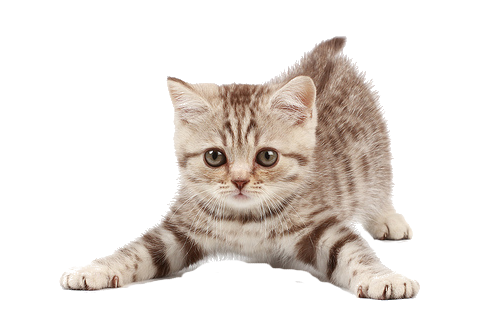
\includegraphics[scale=0.25]{21\21.png}
  \caption{Imagen de un gatito <3 }
  \label{fig:Gatito}
\end{figure}

\section{Matematicas}
Algunas formulas mamalonas:
\begin{itemize}
\item $c^2 = a^2 + b^2$  
\item $x = -b \pm \frag{\sqrt{b^2-4ac}}{2a}$
\end{itemize}

Aqui podemos ver una tabla mamalona ;v
\emph{\textbf{Tabla}}~\ref{tab:Signos}

\begin{table}[h]
  \centering
  \begin{tabular}{| c | c | c |}
    \hline
    Operando & Operando & Resultado\\\hline
    $+$ & $+$ & $+$\\\hline
    $+$ & $-$ & $-$\\\hline
    $-$ & $+$ & $-$\\\hline
    $-$ & $-$ & $+$\\\hline    
  \end{tabular}
  \caption{Signos}
  \label{tab:Signos}
\end{table}


Podemos ver un lindo gatito
\emph{\textbf{Figura}}~\ref{fig:Gatito}
